%!TEX root = ../main.tex


    \color{blue}
    Propuesta: acá poner la gramática y semántica FORMAL del lenguaje de geometría y su simplificación para cadenas binarias

    Todo lo que esté en blue en cap 1, 2, 3 iría en esta parte 1

    Eg:

    Definir  gramáticas   \gramgeo y    \grambin acá y también \mdlbin acá

    Para la semántica de los programas $P$ se puede también usar $\sem{P}$, como hacemos con las fórmulas, pero en este caso, la semántica de un programa es una secuencia en el octágono (o binaria). Habría que definir $\sem{P}$ relativo a un punto inicial $n\in\{0\dots 7\}$ de cómputo: 
    por ejemplo. algo como $\llbracket$\verb#+1#$\rrbracket_n= n+1 \mod 8$.% no me anda usar \verb adentro de \sem :( No deja usar \verb en modo math

    Antes lo llamamos $P(n)$, pero creo que es mejor llamarlo $\sem{P}_n$, asi $\sem{.}$ siempre quiere decir semántica (con fórmulas o secuencias)

    Podemos definir \mdlbinfrag adentro del cap 3 porque es muy particular

    usar este font \verb#[+2]^4# para programas. Ojo, no anda adentro de comando para semántica

    en cap 2 cambié ``la complejidad LoT", ``complejidad LoT", etc por  \mdlbin (es un comando) porque en el contexto de la tesis, quedaba demasiado general hablar de LoT, dado que tenemos varios LoTs

    También cambié  ``complejidad LoT de fragmentos" por  \mdlbinfrag (es un comando)




El desarrollo de un modelo del LoT para la representación de secuencias implica la selección de un conjunto de reglas u operaciones cuya combinación permite la recodificación (sin pérdidas) de cualquier secuencia dada. Introducimos en este capítulo un lenguaje formal para el procesamiento de secuencias que es una variante del \textit{lenguaje de geometría} previamente introducido en~\cite{amalric2017language} para modelar el rendimiento humano de la memoria de trabajo en el dominio espacial. En el mencionado estudio, a los participantes se les presentó una secuencia de ocho ubicaciones un octágono regular. Utilizando datos tanto de comportamiento, como de imágenes cerebrales, se mostró la necesidad y adecuación de un LoT con una sintaxis formal que consta de primitivas geométricas de rotación y simetría, más operaciones de repeticiones con variaciones en el punto de partida o en la cadena resultante~\cite{romano2018bayesian,amalric2017language,f59,f60}\sergio{nosotros}. Se demostró que este lenguaje predice qué secuencias aparecen como regulares y cómo los adultos educados, un pueblo del Amazonas sin educación formal y los niños pequeños se desempeñaban en la tarea explícita de completar las secuencias mostradas~\cite{amalric2017language} o en la tarea implícita de seguimiento ocular de las secuencias~\cite{f60}. La complejidad de la secuencia, definida como una longitud mínima de descripción, también predijo la activación del cerebro humano en un amplio circuito cortical que incluía la corteza frontal inferior justo dorsal al área de Broca~\cite{f60}.

%Our language of geometry enables the generation of programs that can encode any sequence of spatial locations on an octagon. It uses primitive instructions (or rules) regarding the size and the direction of the next step (e.g. +1 = next element clockwise; +2 = second element clockwise), as well as the reflection over some axes (e.g. H = horizontal symmetry, picking the symmetrical location along a horizontal axis). Furthermore, these elements can be repeated, for instance +1^8 describes a full clockwise turn around the octagon (“^8” indicating a repetition of the instruction 8 times). Finally, those repetitions can be arbitrarily embedded (here denoted by brackets). For instance, the expression [[+2]^4]^2<+1> first draws a square, as determined by the subexpression [+2]^4, then a second one (denoted “[…]^2”) with an offset of +1 in the starting point (denoted by “<+1>”; see (58), for a full formal description).

\color{blue}
{\bf a intro o parte I. explicar leng geom, y acá solo de qué forma se reduce para hablar de secuencias. Poner def. formal de leng. geom. en intro o parte I}

El lenguaje de geometría permite la generación de programas que pueden codificar cualquier secuencia de ubicaciones espaciales en un octágono. Utiliza instrucciones primitivas (o reglas) que definen la magnitud y la dirección del siguiente paso (por ejemplo, \verb#+1#= siguiente elemento en el sentido de las agujas del reloj; \verb#+2#= segundo elemento en el sentido de las agujas del reloj), así como la reflexión sobre algunos ejes (por ejemplo, H = simetría horizontal, eligiendo la ubicación simétrica a lo largo de un eje horizontal). Además, estos elementos pueden repetirse, por ejemplo, \verb#+1^8# describe un giro completo en el sentido de las agujas el reloj alrededor del octágono (\verb#^8# indica una repetición de la instrucción 8 veces). Finalmente, estas repeticiones pueden incluirse arbitrariamente (aquí se indica entre paréntesis). Por ejemplo, la expresión \verb#[[+2]^4]^2<+1># primero dibuja un cuadrado, según lo determinado por la subexpresión \verb#[+2]^4#, luego un segundo (\verb#[...]^2#) con un desplazamiento de \verb#+1# en el punto de partida (indicado por \verb#<+1>#). Consultar~\cite{amalric2017language}, para una descripción formal completa. \sergio{Lo incluimos, porque aparece en ambos capítulos}\santi{Sí, de hecho pienso que tendría que ir en el cap. 1 como ejemplo de lenguaje para un dominio específico (secuencias espaciales) y no Turing completo. Se puede apoyar en el octágono que ya tenés dibujado (traer del cap. 2)}

%In the present study, we test the highly constrained hypothesis that the same language, when reduced to only two locations, suffices to account for the human encoding of a completely different type of sequence, namely non-spatial (auditory and visual) binary sequences composed of only two arbitrary states A, B instead of the eight locations of the octagon. For such sequences, the language can be stripped of most of its primitives. We kept only the operations of staying (“+0”), moving to the other item (here denoted “b”, i.e. the alternation instruction, but equivalent to +4 or point symmetry in the original octagon-based language), and repetition (“^n”, where n is any number), possibly with a variation in the starting point (denoted by <x> where x is an elementary instruction, either +0 or b). As already mentioned, embedding of expressions is represented by brackets (“[….]”) and concatenation by commas (“,”). The language is thus able to encode any arbitrary repetition of instructions in a compressed manner. The sequence AAAA, for instance, would be denoted [+0]^4 (i.e. stay in the same state four times), the sequence ABAB would be denoted [+0]^4<b> (four repetitions, with an item change after each one; i.e., four alternations). The language is recursive and can produce nested descriptions; AABAAB can be described as “two repetitions of [two repetitions plus one change]” (see examples in Figure 1A). Because of recursion, even long sequences can be encoded compactly in an easy-to-remember form; ABABABBBBBBBABABABBBBBBB is “2 times [5 alternations and 5 repetitions]”. The code is available online at \hyperref[https://github.com/sromano/language-of-geometry]{https://github.com/sromano/language-of-geometry}


En el presente estudio, probamos la hipótesis de que el mismo lenguaje, cuando se reduce a sólo dos ubicaciones, es suficiente para dar cuenta de la codificación humana en un tipo completamente diferente de secuencias: un dominio no espacial (auditivo y visual) de secuencias binarias compuestas por sólo dos estados arbitrarios A y B en lugar de las ocho ubicaciones del octágono. Para tales secuencias, el lenguaje puede ser despojado de la mayoría de sus primitivas. Sólo mantuvimos las operaciones de permanecer (\verb#+0#), pasar al otro elemento (aquí denotado \verb#B#, es decir, la instrucción de alternancia, pero equivalente a \verb#+4# o simetría de puntos en el lenguaje original del octágono) y repetición (\verb#^N#, donde \verb#N# es cualquier número natural), con la posibilidad de incluir una variación en el punto de inicio (denotado por \verb#<X># donde \verb#X# es una instrucción primitiva, ya sea \verb#+0# o \verb#B#). Como ya se mencionó, el anidamiento de expresiones se representa con corchetes (\verb#[...]#) y la concatenación con comas (\verb#...,...#). Por tanto, el lenguaje puede codificar cualquier repetición arbitraria de instrucciones de forma comprimida. \santi{Dado que es una tesis en computación, tiene sentido dar una semántica formal de este lenguaje. Me imagino que podría ser un recorte de lo que habrás puesto en la intro sobre Leng geometría.} La secuencia AAAA, por ejemplo, se denotaría \verb#[+0]^4# (es decir, permanecería en el mismo estado cuatro veces), la secuencia ABAB se denotaría \verb#[+0]^4<B># (cuatro repeticiones, con un cambio de elemento después de cada una, es decir, cuatro alternancias). El lenguaje es recursivo y puede producir descripciones anidadas; AABAAB puede ser descrito como ``dos repeticiones de [dos repeticiones más un cambio]'' (véase el Ejemplo en la Figura~\ref{PlosBIO-F1}A). Debido a la recursión, incluso secuencias largas pueden ser codificadas de manera compacta en un formato fácil de recordar: ``ABABABBBBBABABABBBBB'' es ``2 repeticiones de [5 alternaciones y 5 repeticiones]''. El código se encuentra disponible en \hyperref[https://github.com/sromano/language-of-geometry]{\url{https://github.com/sromano/language-of-geometry}}


%Given this language of thought, for each sequence, one can find the simplest expression that describes it, and its associated complexity level (analogous to KC). Complexity is calculated by as a weighted sum of the fixed cost attached to each primitive instruction (+0, and b). As in our previous work (58), the additional cost for repeating an instruction n times is assumed to correspond to log10(n) (rounded up), i.e. the number of digits needed to encode the number in decimal notation. The relative value of those two costs is such that even a single repetition compresses an expression: +0^2 is assumed to be more compressed than the mere concatenation of +0+0 (see supporting information in ref. 56 for details). As a result, the language favors an abstract description of sequences based on the maximum amount of nested repetitions, thus sharply dissociating sequence length and complexity. Among the multiple expressions that can describe the same sequence, the expression (or in some cases, the multiple expressions) with the lowest complexity is thought to correspond to the human mental representation of the sequence. In a nutshell, the assumption is that, in order to minimize memory load, participants mentally compress the sequence structure using the proposed formal language. The use of a minimal number of unitary operations, as well as the selection of the shortest representation, is in accordance with a simplicity principle, proposed as an essential component of learning, which states that the simplest hypothesis should be favored (32,55).The low impact of length on LoT complexity makes it markedly different from other metrics such as algorithmic complexity (43,44,46), for which longer sequences are systematically considered more complex since they are far less probable (even if longer by only one item). Although other complexity measures, such as change complexity, are correlated with ours, as further described below, they may also differ substantially for long sequences that can be hierarchically represented (e.g., AAABBB has the same LoT complexity as AAABBBAAABBB, since both are captured by a formula with two instructions and two digits, while change complexity is three times greater for the latter than for the former). Thus, the existing theories make distinct predictions, and it should be possible to empirically decide which one provides the best fit to human sequence memory abilities.

Teniendo en cuenta este LoT, para cada secuencia, uno puede encontrar la expresión más simple que lo describa y su complejidad asociada (análoga a CK). La complejidad es calculada como una suma ponderada por el costo fijo asociada a cada primitiva (\verb#+0# y \verb#B#). Como en el lenguaje original~\cite{amalric2017language}, el costo adicional de repetir una instrucción $n$ veces corresponde a $\lceil \log_{10} n \rceil$, es decir, el número de dígitos necesarios para codificar el número en notación decimal. El valor relativo de esos dos costos es tal que incluso una sola repetición comprime una expresión: \verb#+0^2# se supone que es una expresión más comprimida que la simple concatenación de \verb#+0,+0# (ver información en~\cite{amalric2017language} para detalles). Como resultado, el lenguaje favorece una descripción abstracta de secuencias basada en en la cantidad máxima de repeticiones anidadas, disociando de manera fuerte la longitud de una secuencia con su complejidad.
\color{black}

--------------------------------------------------------

\paragraph{La gramática \gramgeo.}
Definimos la gramática para el {\em lenguaje de geometría} $\grambool$ del siguiente modo:

\begin{center}
\begin{tabular}{cc}

    \begin{minipage}[t]{0.35\textwidth}
    {\bf Símbolo inicial}

    \medskip

    \begin{tabular}{rcl}
    \start & $\to$ & \verb#[#\inst\verb#]# %& símbolo inicial 
    \end{tabular}

    \bigskip

    {\bf Producciones básicas}

    \medskip

    \begin{tabular}{rcl}
    \inst  & $\to$ & \atom %& producción atómica 
    \\
    \inst  & $\to$ & \inst\verb#,#\inst %& concatenación 
    \\
    \inst  & $\to$ & \rep\verb#[#\inst\verb#]^#$k$%& familia repetir con $n \in [2,8]$ 
    \\
    \rep  & $\to$ & \verb#REP0# %& repetición simple 
    \\

    \rep  & $\to$ & \verb#REP1<#\atom\verb#># %& repetir con variación del punto de inicio usando ATOMIC
    \\
    \rep  & $\to$ & \verb#REP2<#\atom\verb#># %& repetir con variación de la secuencia resultante usando ATOMIC
    \\
    \end{tabular}
    \end{minipage}
    
    \begin{minipage}[t]{0.35\textwidth}

    {\bf Producciones atómicas}

    \medskip

    \begin{tabular}{rcl}
    \atom  & $\to$ & \verb#-1# %& siguiente elemento en sentido antihorario (ACW) 
    \\
    \atom  & $\to$ & \verb#-2# %& segundo elemento ACW 
    \\
    \atom  & $\to$ & \verb#-3# %& tercer elemento ACW 
    \\
    \atom  & $\to$ & \verb#+0# %& permanecer en la misma posición 
    \\
    \atom  & $\to$ & \verb#+1# %& siguiente elemento en sentido horario (CW)
    \\
    \atom  & $\to$ & \verb#+2# %& segundo elemento CW 
    \\
    \atom  & $\to$ & \verb#+3# %& tercer elemento CW 
    \\
    \atom  & $\to$ & \verb#A # %& simetría alrededor de un eje diagonal 
    \\
    \atom  & $\to$ & \verb#B # %& simetría alrededor del otro eje diagonal 
    \\
    \atom  & $\to$ & \verb#H # %& simetría horizontal 
    \\
    \atom  & $\to$ & \verb#V # %& simetría vertical 
    \\
    \atom  & $\to$ & \verb#P # %& simetría rotacional 
    \end{tabular}
    \end{minipage}
\end{tabular}
\end{center}

\noindent donde $k$ es la representación en decimal de un número natural en el intervalo $\{2,\dots,8\}$.


Los {\em programas} de \gramgeo serán las palabras del lenguaje definido por \gramgeo. Usaremos indistintamente \gramgeo para referirnos a la gramática o al lenguaje que representa (quedando siempre claro del contexto cuál de las dos aplica).

\paragraph{La semántica de \gramgeo.}
Los programas por sí solos no tienen semántica, sino que la semántica viene dada por un par $(P,n)$, donde $P$ es un programa de \gramgeo y $n$ es un número natural entre 0 y 7. Denotaremos con $\sem{P}_n$ a la semántica de tal par, y será una secuencia no vacía de números naturales sobre el alfabeto $\{0,\dots,7\}$. Intuitivamente, $\sem{P}_n$ representa o describe un camino  en el octágono de la Figura \ref{fig:circle}, cuando se `ejecuta' $P$ a partir del punto $n$. El mismo programa $P$ podrá describir distintas secuencias dependiendo del valor de $n$. 
\widesanti{ACA ALGO MAS DE BLA BLA INTUITIVO}

\begin{figure}[ht]
\begin{center}
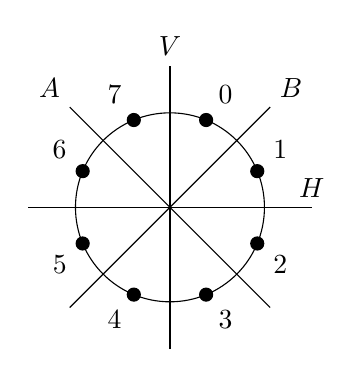
\begin{tikzpicture}[scale=.6]
\draw (-3,0) -- (3,0) node[above]{$H$};
\draw (0,-3) -- (0,3) node[above]{$V$};
\draw (-2.121320344,-2.121320344) -- (2.121320344,2.121320344) node[above right]{$B$};
\draw (2.121320344, -2.121320344) -- (-2.121320344,2.121320344) node[above left]{$A$};
\node at (0.765366865,  1.847759065) [circle,draw, scale=.5, fill, label=67.5:$0$]{};
\node at (1.847759065   , 0.765366865) [circle,draw, scale=.5, fill, label=22.5:$1$]{};
\node at (1.847759065   , -0.765366865) [circle,draw, scale=.5, fill, label=-22.5:$2$]{};
\node at (0.765366865   , -1.847759065) [circle,draw, scale=.5, fill, label=-67.5:$3$]{};
\node at (-0.765366865, -1.847759065) [circle,draw, scale=.5, fill, label=-112.5:$4$]{};
\node at (-1.847759065, -0.765366865) [circle,draw, scale=.5, fill, label=-157.5:$5$]{};
\node at (-1.847759065, 0.765366865) [circle,draw, scale=.5, fill, label=-202.5:$6$]{};
\node at (-0.765366865, 1.847759065) [circle,draw, scale=.5, fill, label=-247.5:$7$]{};
\draw (0,0) circle (2cm);
\end{tikzpicture}
\end{center}
   \caption{El octógono sobre el que \gramgeo describe caminos}\label{fig:circle}
\end{figure}

Se puede ver de la definición de la gramática \gramgeo que un programa $P$ será siempre de la forma 

\begin{center}
$P=$\verb#[# $I_1$ \verb#,# \dots \verb#,# $I_\ell$ \verb#]#
\end{center}

\noindent donde las $I_i$ serán {\em instrucciones} derivadas de \inst. Por comodidad, definiremos también la semántica sobre el conjunto de de instrucciones, es decir definiremos $\sem{I}_n$, donde $I$ es una instrucción. Una {\em instrucción atómica} es cualquiera derivada del símbolo \atom\ en la gramática \gramgeo.

La definición de la semántica formal la veremos más adelante. 
Por ahora veamos informalmente la semántica de cada instrucción atómica: 
\begin{itemize}
\item \verb#-1# representa siguiente elemento en sentido antihorario (SAH)

\item \verb#-2# representa el segundo elemento SAH

\item \verb#-3# representa el tercer elemento SAH 

\item \verb#+0# representa permanecer en la misma posición

\item \verb#+1# representa el siguiente elemento en sentido horario (SH)
 
\item \verb#+2# representa el segundo elemento SH

\item \verb#+3# representa el tercer elemento SH 

\item \verb#A# representa la simetría sobre un eje diagonal

\item \verb#B# representa la simetría sobre el otro eje diagonal 

\item \verb#H# representa la simetría horizontal 

\item \verb#V# representa la simetría vertical 

\item \verb#P# representa la simetría rotacional 
\end{itemize}

Además, \gramgeo tiene tres formas de repeticiones de (sub)programas:

\begin{itemize}
\item Si $P=$\verb#[# $I_1$ \verb#,# \dots \verb#,# $I_\ell$ \verb#]# es un programa, la ejecución de \verb#REP0#$P$\verb#^#$k$ desde $n$ será equivalente a la ejecución del siguiente programa desde $n$: 
\begin{center}
\verb#[# $I_1$ \verb#,# \dots \verb#,# $I_\ell$ \verb#,# 
         $I_1$ \verb#,# \dots \verb#,# $I_\ell$ \verb#,#
         $\dots$ \verb#,# 
         $I_1$ \verb#,# \dots \verb#,# $I_\ell$ \verb#]#
\end{center} ESTO NO SE SI ESTA BIEN
que tiene $k$ copias de $P$.
\noindent Por ejemplo...



\item Si $A$ es una instrucción atómica y $P$ es un programa, la ejecución del programa 
\verb#REP1<#$A$\verb#>#$P$\verb#^#$k$ desde $n$ será...

\item Si $A$ es una instrucción atómica y $P$ es un programa, la ejecución del programa 
\verb#REP2<#$A$\verb#>#$P$\verb#^#$k$ desde $n$ será...

\end{itemize}

Dado $\alpha$ un programa o una instrucción, y dado $n\in\{0,\dots,7\}$, definimos ahora formalmente $\sem{\alpha}_n$, la {\em semántica de $\alpha$ a partir de $n$}, recursivamente en la complejidad del árbol sintáctico de $\alpha$ en la gramática \gramgeo.

Definimos primero la semántica de las instrucciones atómicas de la siguiente forma:

\begin{tabular}{cc}
    \begin{minipage}[t]{0.45\textwidth}
        \begin{itemize}
        \item $\llbracket$\verb#+0#$\rrbracket_n  \eqdef  n$ 
        \item $\llbracket$\verb#+1#$\rrbracket_n  \eqdef  n+1 \mod 8$  
        \item $\llbracket$\verb#-1#$\rrbracket_n  \eqdef  n-1 \mod 8$  
        \item $\llbracket$\verb#+2#$\rrbracket_n  \eqdef  n+2 \mod 8$  
        \item $\llbracket$\verb#-2#$\rrbracket_n  \eqdef  n-2 \mod 8$  
        \item $\llbracket$\verb#+3#$\rrbracket_n  \eqdef  n+3 \mod 8$  
        \item $\llbracket$\verb#-3#$\rrbracket_n  \eqdef  n-3 \mod 8$  
        \end{itemize}
    \end{minipage}
    &
    \begin{minipage}[t]{0.45\textwidth}
        \begin{itemize}
        \item $\llbracket$\verb#P#$ \rrbracket_n  \eqdef  4+n \mod 8$  
        \item $\llbracket$\verb#H#$ \rrbracket_n  \eqdef  3-n \mod 8$  
        \item $\llbracket$\verb#V#$ \rrbracket_n  \eqdef  7-n \mod 8$  
        \item $\llbracket$\verb#A#$ \rrbracket_n  \eqdef  5-n \mod 8$  
        \item $\llbracket$\verb#B#$ \rrbracket_n  \eqdef  1-n \mod 8$  
        \end{itemize}
    \end{minipage}
\end{tabular}

\medskip

La semántica de las otras instrucciones (salvo la regla de que introduce `\verb#,#') es la siguiente:
\begin{itemize}
\item Si $I=$ \verb#REP0#$P$\verb#^#$k$, con $P$ un programa, 
definimos 
$\sem{I}_n$......


\item Si $I=$ \verb#REP1<#$A$\verb#>#$P$\verb#^#$k$, con $P$ un programa y $A$ una instrucción atómica, 
definimos 
$\sem{I}_n$......

\item Si $I=$ \verb#REP2<#$A$\verb#>#$P$\verb#^#$k$, con $P$ un programa y $A$ una instrucción atómica, 
definimos 
$\sem{I}_n$......
\end{itemize}

Finalmente, si $P=$ \verb#[# $I$ \verb#]#, entonces $\sem{P}_n\eqdef\sem{I}_n$, y si
\begin{center}
$P=$\verb#[# $I_1$ \verb#,# $I_2$ \verb#,# \dots \verb#,# $I_\ell$ \verb#]#
\end{center}
con $\ell>1$,
entonces

\begin{center}
$\sem{P}_n \eqdef \sem{I_1}_n \concat \llbracket$
\verb#[# $I_2$ \verb#,# \dots \verb#,# $I_\ell$ \verb#]#
$\rrbracket_m$
\end{center}

\noindent donde $m\in\{0,\dots,7\}$ es el último símbolo de la secuencia $\sem{I_1}_n$ y $\cdot\concat\cdot$ representa la concatenación de secuencias.


\paragraph{Complejidad para \gramgeo.} 
Si $\alpha$ es un programa o una instrucción de \gramgeo, definimos el {\em tamaño} de $\alpha$, notado $|\alpha|$ de la siguiente manera:
%
\begin{itemize}
\item Si $\alpha$ es una instrucción atómica, $|\alpha|\eqdef 2$.

\item Si $\alpha$ es una instrucción de la forma 
\verb#REP0#$P$\verb#^#$k$, con $P$ un programa, 
entonces $|\alpha|\eqdef |P|+\lceil \log k\rceil$.

\item Si $\alpha$ es una instrucción de la forma 
\verb#REP1<#$A$\verb#>#$P$\verb#^#$k$ o de la forma 
\verb#REP1<#$A$\verb#>#$P$\verb#^#$k$ 
con $P$ un programa y $A$ una instrucción atómica, 
entonces $|\alpha|\eqdef |P|+\lceil \log k\rceil+|A|$.

\item Si $\alpha$ es un programa de la forma
\verb#[# $I_1$ \verb#,# $I_2$ \verb#,# \dots \verb#,# $I_\ell$ \verb#]#
entonces $|\alpha|\eqdef \sum_{i=1}^\ell|I_i|$.
\end{itemize}
%
Si $s$ es una secuencia no vacía sobre $\{0,\dots,7\}$, definimos la {\em $\gramgeo$-complejidad de la descripción mínima} de $s$, notada $\mdlgeo(s)$, como el tamaño del programa que, ejecutado desde 0, produce la secuencia $s$, es decir,
$$
\mdlgeo(s)\eqdef\min\{|P|\mid P\in\gramgeo,\sem{P}_0=s\}.
$$
Por ejemplo, ..............
